\chapter{Code Implementation Details}

This chapter provides a deep dive into the implementation. We use object-oriented programming to keep the codebase modular and testable.

\section{Translation Service}
File: \texttt{src/translation.py}

The `TranslationService` class encapsulates the complexity of the NLLB model. 

\begin{lstlisting}[language=Python, caption=Initializing NLLB]
class TranslationService:
    def __init__(self, model_name="facebook/nllb-200-distilled-600M"):
        # We check for GPU availability automatically
        self.device = 0 if torch.cuda.is_available() else -1
        
        print(f"Loading Translation Model: {model_name}...")
        self.tokenizer = AutoTokenizer.from_pretrained(model_name)
        self.model = AutoModelForSeq2SeqLM.from_pretrained(model_name)
        
        if self.device == 0:
            self.model = self.model.to("cuda")
\end{lstlisting}

\subsection{Handling Multilingual Inputs}
The core challenge with NLLB is that it requires a "Forced BOS Token" (Beginning of Sentence) to know which language to translate \textit{into}.

\begin{lstlisting}[language=Python, caption=Forcing English Output]
    def translate(self, text, target_lang="eng_Latn"):
        if not text: return ""

        # 1. Tokenize Input
        inputs = self.tokenizer(text, return_tensors="pt", padding=True)
        if self.device == 0:
            inputs = {k: v.to("cuda") for k, v in inputs.items()}

        # 2. Force Target Language Token
        # "eng_Latn" is the NLLB code for English
        forced_bos = self.tokenizer.convert_tokens_to_ids(target_lang)
        
        # 3. Generate
        with torch.no_grad():
            tokens = self.model.generate(
                **inputs, 
                forced_bos_token_id=forced_bos, 
                max_length=512
            )
            
        # 4. Decode
        return self.tokenizer.batch_decode(tokens, skip_special_tokens=True)[0]
\end{lstlisting}

\section{Summarization Service}
File: \texttt{src/summarization.py}

The summarizer is simpler because we leverage the Hugging Face `pipeline` abstraction.

\begin{lstlisting}[language=Python]
class SummarizationService:
    def __init__(self):
        # Pipelines handle tokenization, device placement, and decoding internally
        self.summarizer = pipeline("summarization", model="facebook/bart-large-cnn")

    def summarize(self, text):
        # We set tight constraints on length to ensure concise outputs
        result = self.summarizer(
            text, 
            max_length=130,  # Max summary length
            min_length=30,   # Min summary length
            do_sample=False  # Deterministic output
        )
        return result[0]['summary_text']
\end{lstlisting}

\section{The Application Controller}
File: \texttt{app.py}

Finally, we tie everything together. 

\begin{figure}[H]
    \centering
    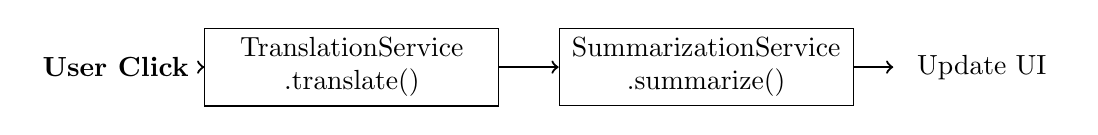
\begin{tikzpicture}[node distance=3cm]
        \node[font=\bfseries, align=center, text width=2cm] (start) {User Click};
        \node[right of=start, draw, align=center, text width=3.5cm] (t) {TranslationService \\ .translate()};
        \node[right of=t, draw, align=center, text width=3.5cm, xshift=1.5cm] (s) {SummarizationService \\ .summarize()};
        \node[right of=s, align=center, text width=2cm, xshift=0.5cm] (end) {Update UI};
        
        \draw[->, thick] (start) -- (t);
        \draw[->, thick] (t) -- (s);
        \draw[->, thick] (s) -- (end);
    \end{tikzpicture}
    \caption{Execution Flow}
\end{figure}

The \texttt{app.py} script initializes these services once (globally) so they don't reload on every request, which would be very slow.
